\documentclass[aspectratio=169,10pt]{beamer}
\usetheme{Madrid}\setbeamertemplate{navigation symbols}{}
\title{Intrinsic Timing and Position Reconstruction with Adjacent SiPMs}
\subtitle{Fourth- and Twentieth-Detected-Hit Timing, Local Position Reconstruction and EndTop Context}
\author{René Ríos Torres}\institute{Universidad de La Serena}
\begin{document}\frame{\titlepage}\newcommand{\SlopeFourPE}{5.880}
\newcommand{\SlopeTwentyPE}{9.673}
\newcommand{\SigmaXFourPE}{13.34}
\newcommand{\SigmaXTwentyPE}{10.32}
\newcommand{\EffFourPE}{1.000}
\newcommand{\EffTwentyPE}{1.000}

\begin{frame}{Scientific questions}
\begin{itemize}
\item EXEC 11 4PE reproduction gate: \textbf{PASS}.
\item Native and matched samples coincide: 4PE and 20PE efficiencies are 100\%.
\item 20th-hit differential width: 99.8 ps, versus 78.5 ps for 4th hit.
\item Cross-validated X RMS68: 10.32 mm at 20PE, versus 13.34 mm at 4PE.
\item Higher thresholds improve X RMS68 here, while calibration nonlinearity rises.
\item Intrinsic simulation prediction; 20th detected hit is not waveform 20\% CFD.
\end{itemize}
\end{frame}
\begin{frame}{Detector and fine scan}
\centering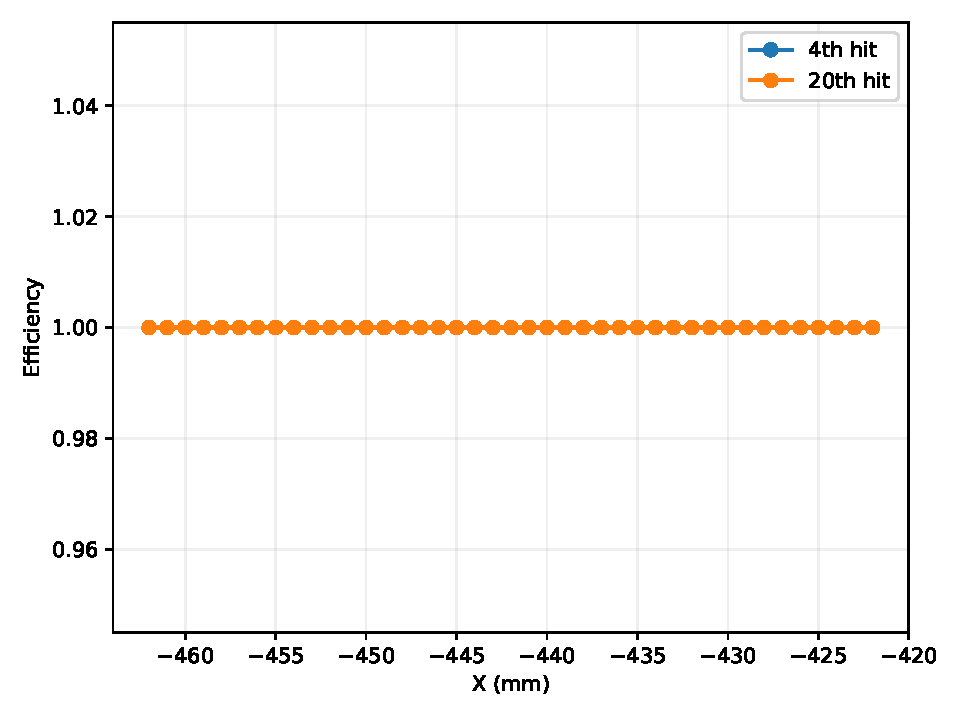
\includegraphics[width=.88\textwidth,height=.72\textheight,keepaspectratio]{../figures/efficiency_4_20_vs_x.pdf}
\end{frame}
\begin{frame}{Available datasets}
\centering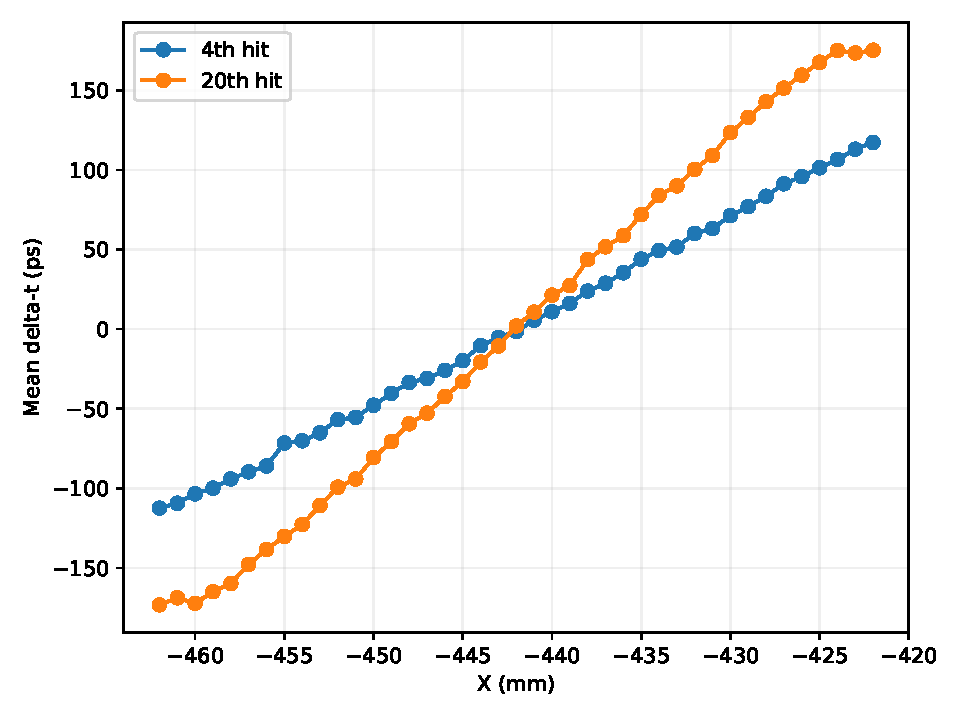
\includegraphics[width=.88\textwidth,height=.72\textheight,keepaspectratio]{../figures/mean_delta_4_20_vs_x.pdf}
\end{frame}
\begin{frame}{From hits to observables}
\centering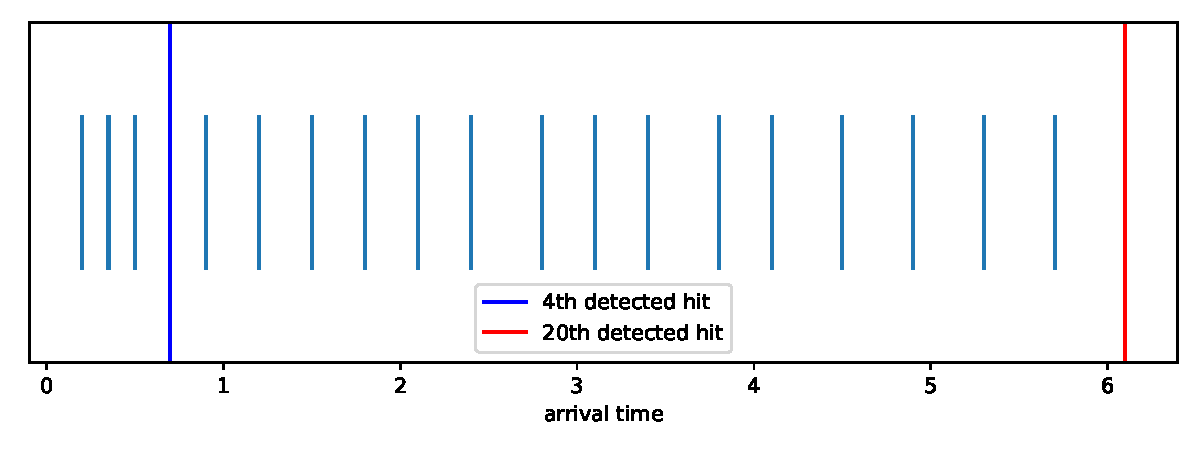
\includegraphics[width=.88\textwidth,height=.72\textheight,keepaspectratio]{../figures/order_statistic_schematic.pdf}
\end{frame}
\begin{frame}{Ordered photon arrivals}
\centering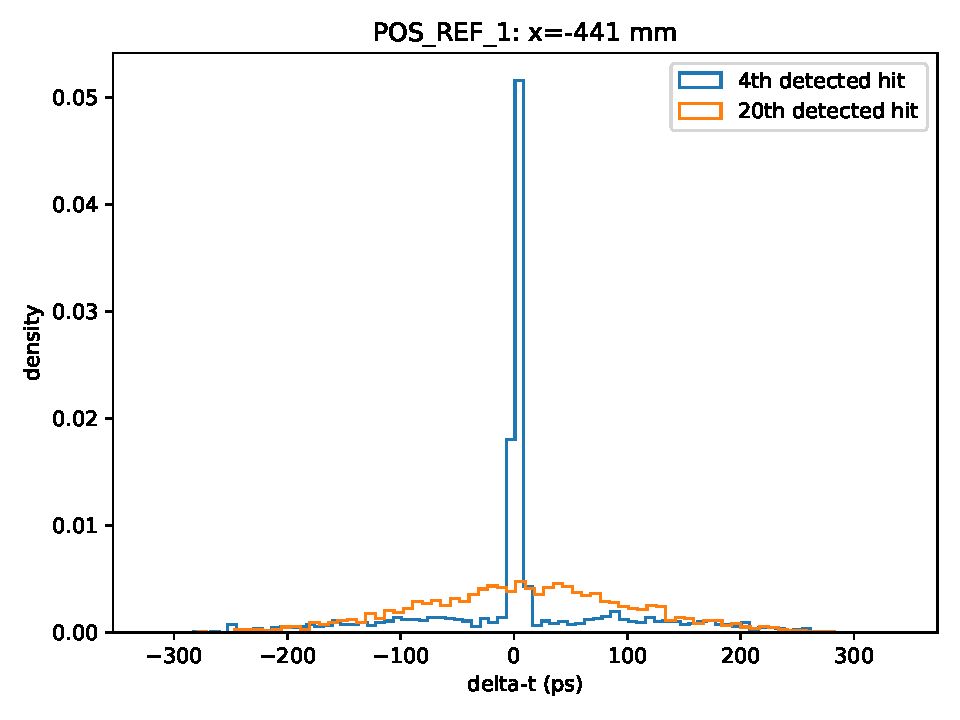
\includegraphics[width=.88\textwidth,height=.72\textheight,keepaspectratio]{../figures/pos_ref_1_delta_t_4_20.pdf}
\end{frame}
\begin{frame}{Critical distinction: 20th hit is not 20 percent CFD}
\Large 20th detected-hit timing $\neq$ 20\% constant-fraction timing.\par\medskip Order statistic versus waveform threshold; one pair versus 64-channel combination.
\end{frame}
\begin{frame}{Common and differential timing}
\centering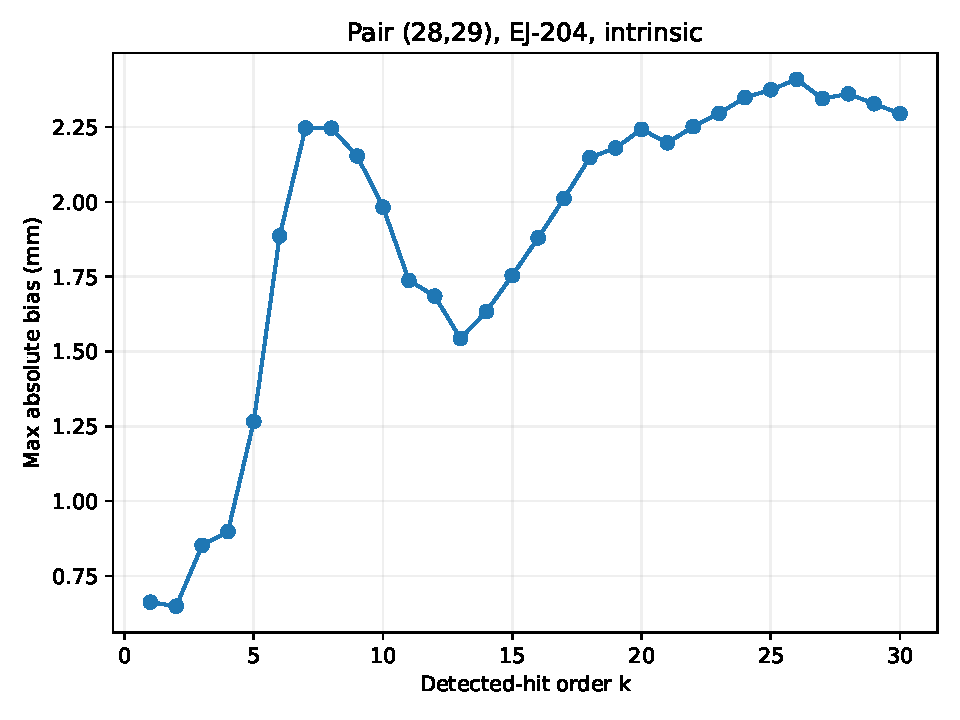
\includegraphics[width=.88\textwidth,height=.72\textheight,keepaspectratio]{../figures/threshold_bias.pdf}
\end{frame}
\begin{frame}{Native versus matched samples}
\centering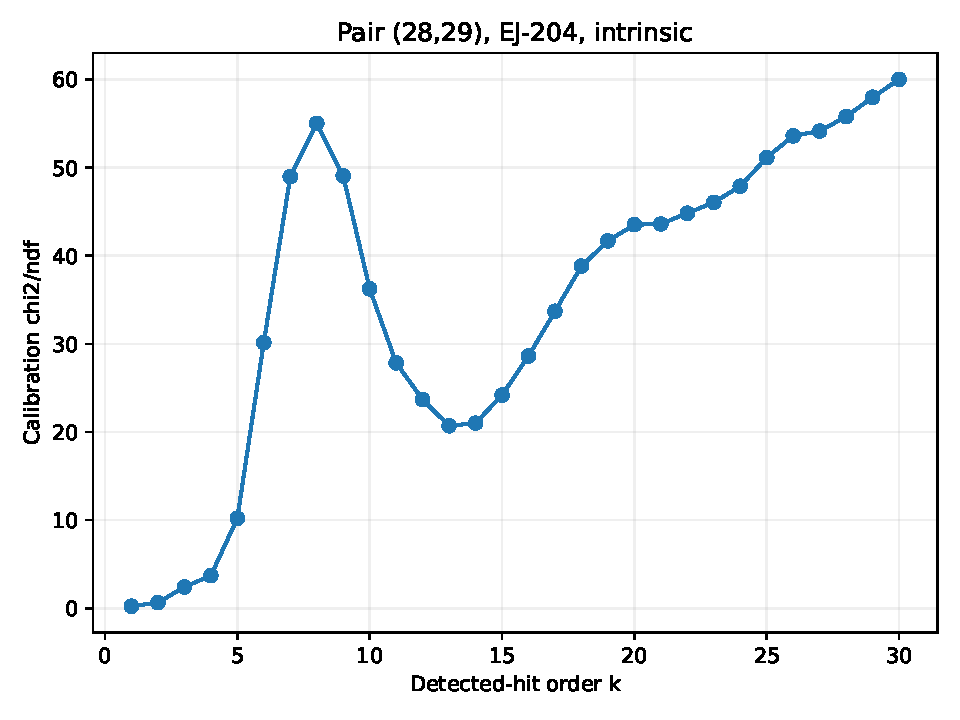
\includegraphics[width=.88\textwidth,height=.72\textheight,keepaspectratio]{../figures/threshold_chi2.pdf}
\end{frame}
\begin{frame}{4PE reproduction gate}
\centering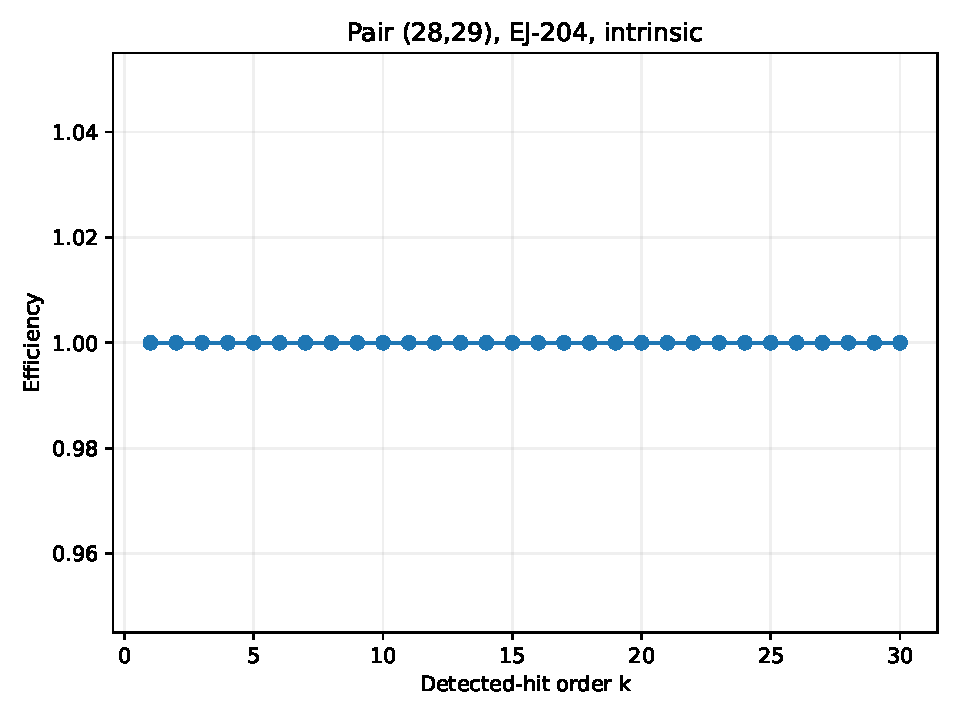
\includegraphics[width=.88\textwidth,height=.72\textheight,keepaspectratio]{../figures/threshold_efficiency.pdf}
\end{frame}
\begin{frame}{Raw temporal response}
\centering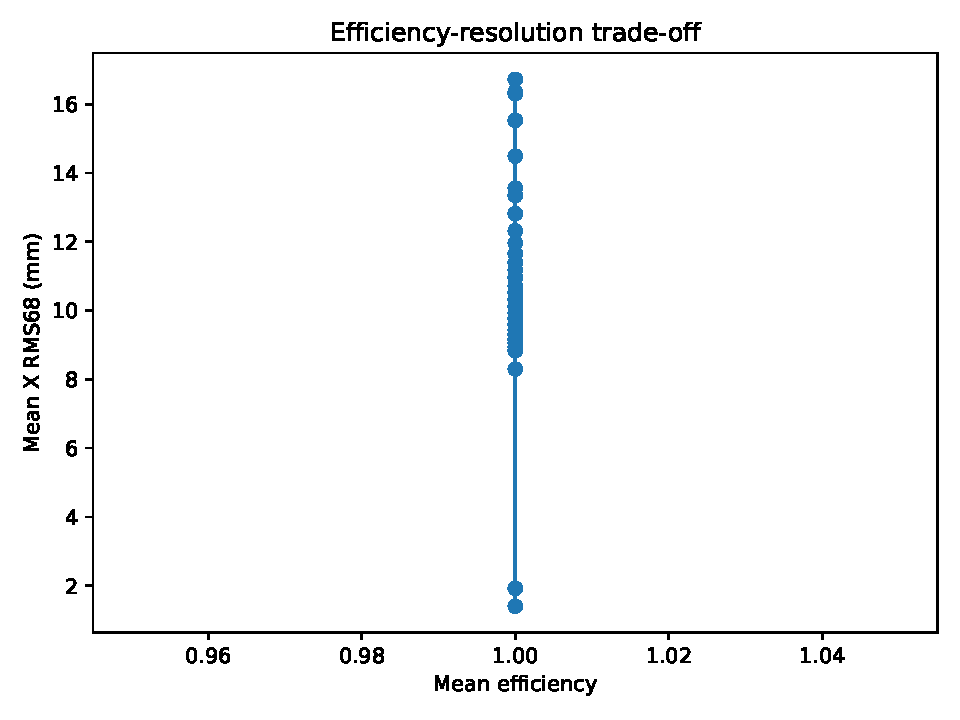
\includegraphics[width=.88\textwidth,height=.72\textheight,keepaspectratio]{../figures/threshold_pareto.pdf}
\end{frame}
\begin{frame}{Efficiency versus X}
\centering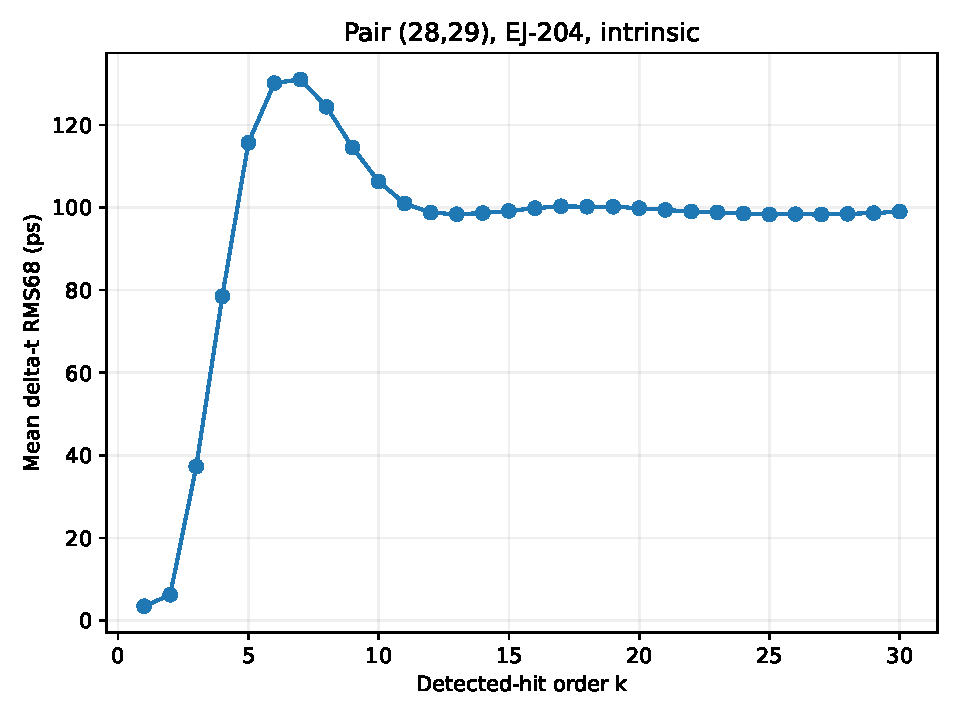
\includegraphics[width=.88\textwidth,height=.72\textheight,keepaspectratio]{../figures/threshold_sigma_dt.pdf}
\end{frame}
\begin{frame}{Mean differential time}
\centering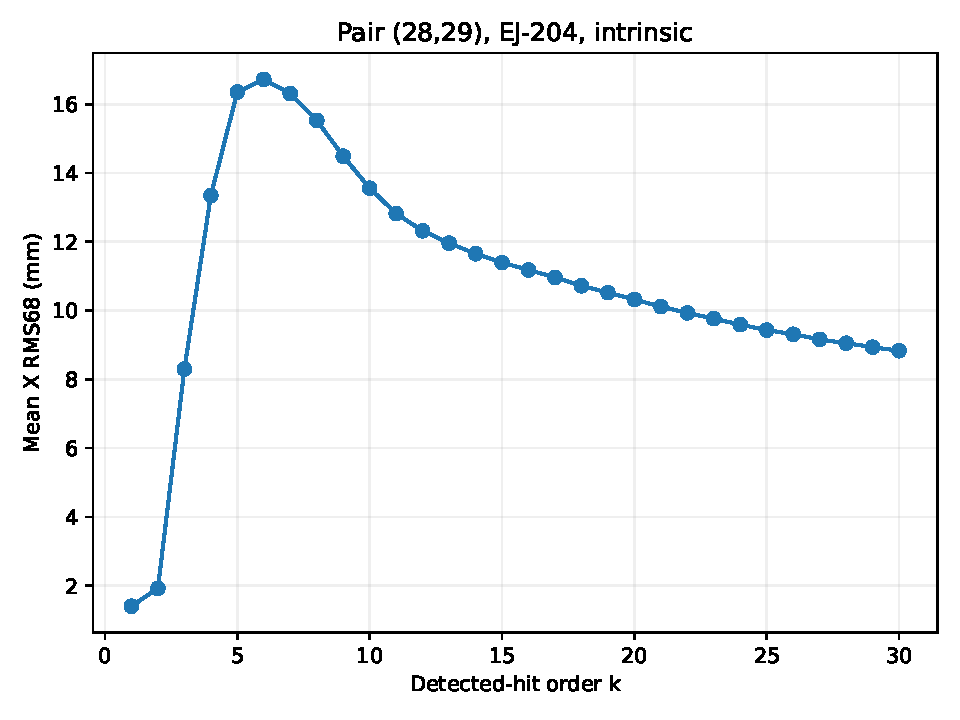
\includegraphics[width=.88\textwidth,height=.72\textheight,keepaspectratio]{../figures/threshold_sigma_x.pdf}
\end{frame}
\begin{frame}{Timing width versus X}
\centering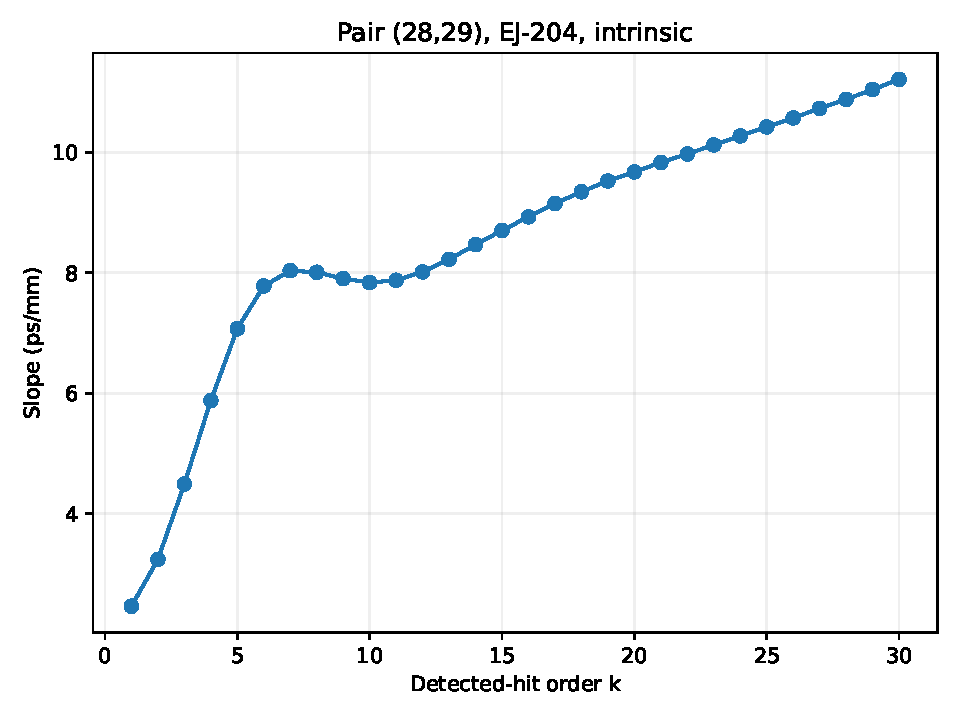
\includegraphics[width=.88\textwidth,height=.72\textheight,keepaspectratio]{../figures/threshold_slope.pdf}
\end{frame}
\begin{frame}{A-B correlation}
\centering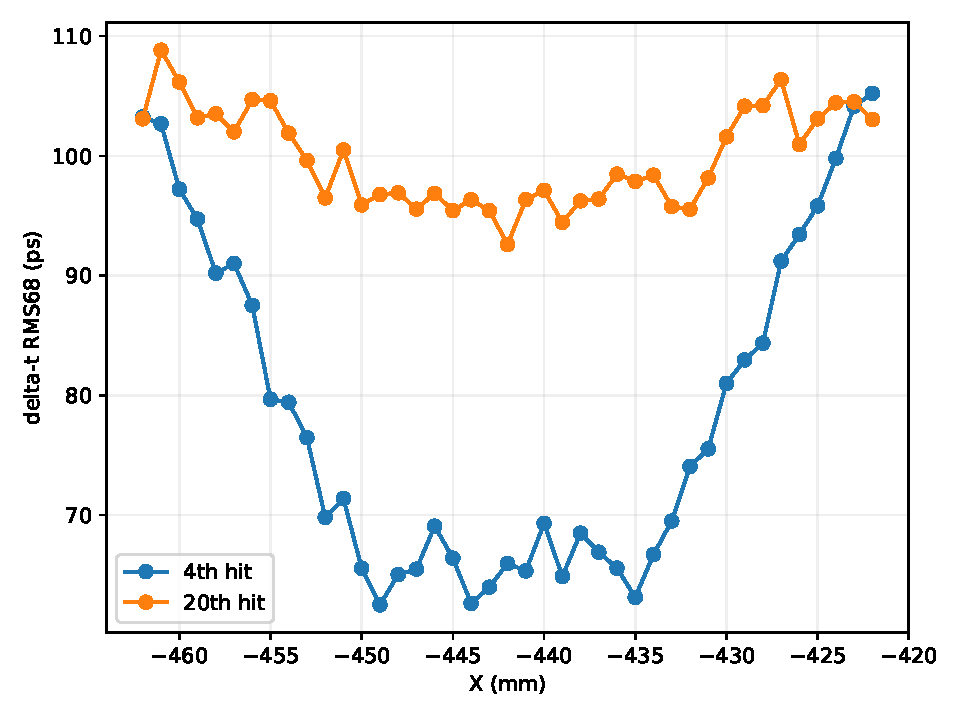
\includegraphics[width=.88\textwidth,height=.72\textheight,keepaspectratio]{../figures/timing_width_4_20_vs_x.pdf}
\end{frame}
\begin{frame}{4PE calibration}
\centering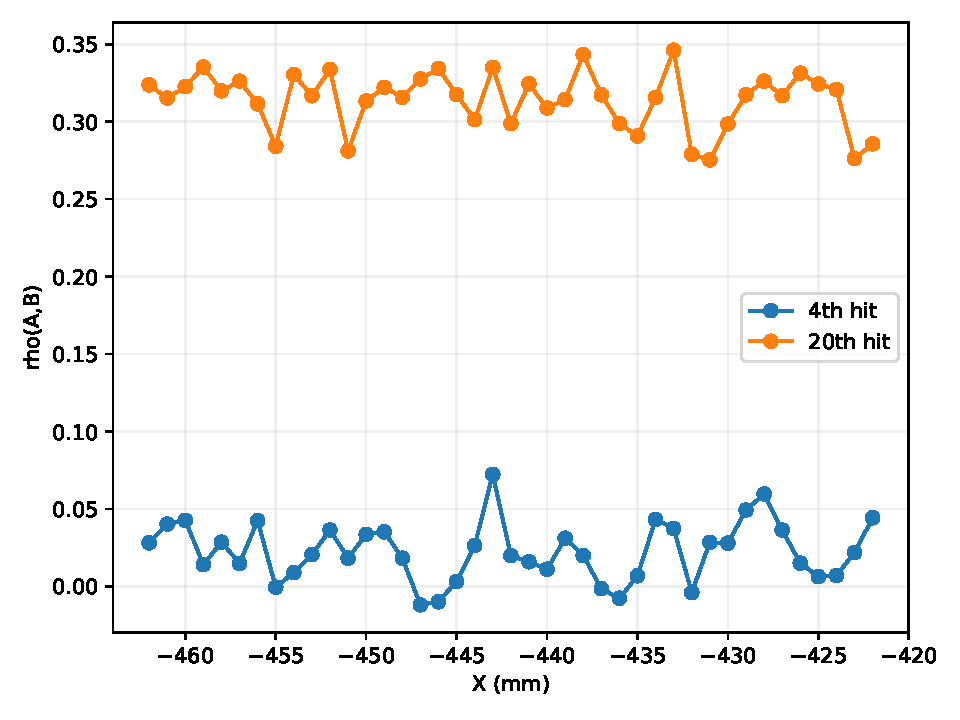
\includegraphics[width=.88\textwidth,height=.72\textheight,keepaspectratio]{../figures/correlation_ab_vs_x.pdf}
\end{frame}
\begin{frame}{20PE calibration}
\centering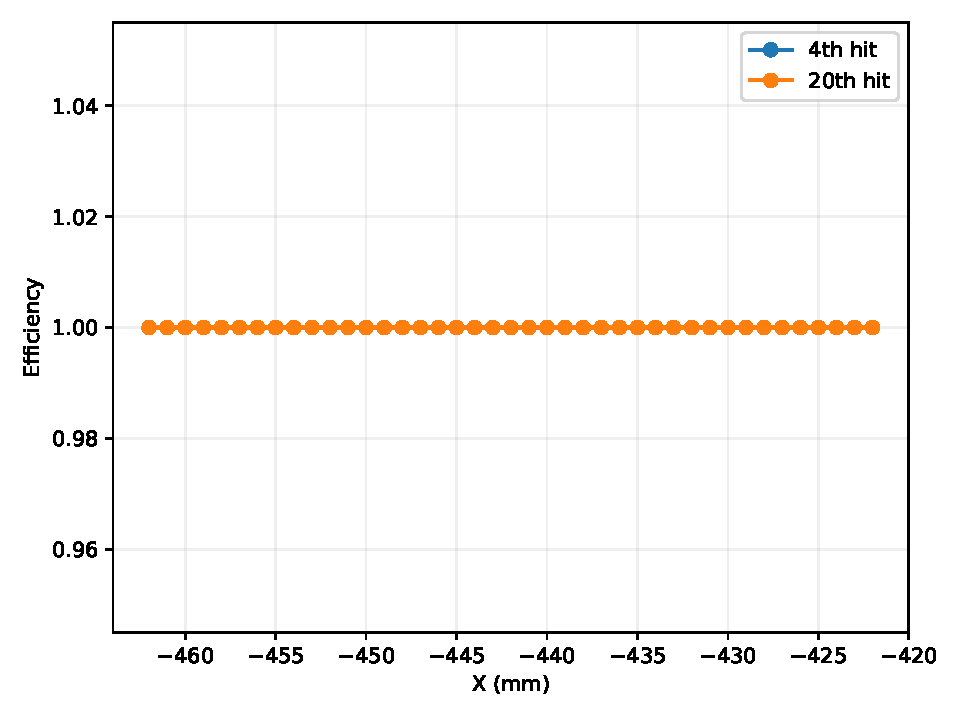
\includegraphics[width=.88\textwidth,height=.72\textheight,keepaspectratio]{../figures/efficiency_4_20_vs_x.pdf}
\end{frame}
\begin{frame}{Slope and effective velocity}
\centering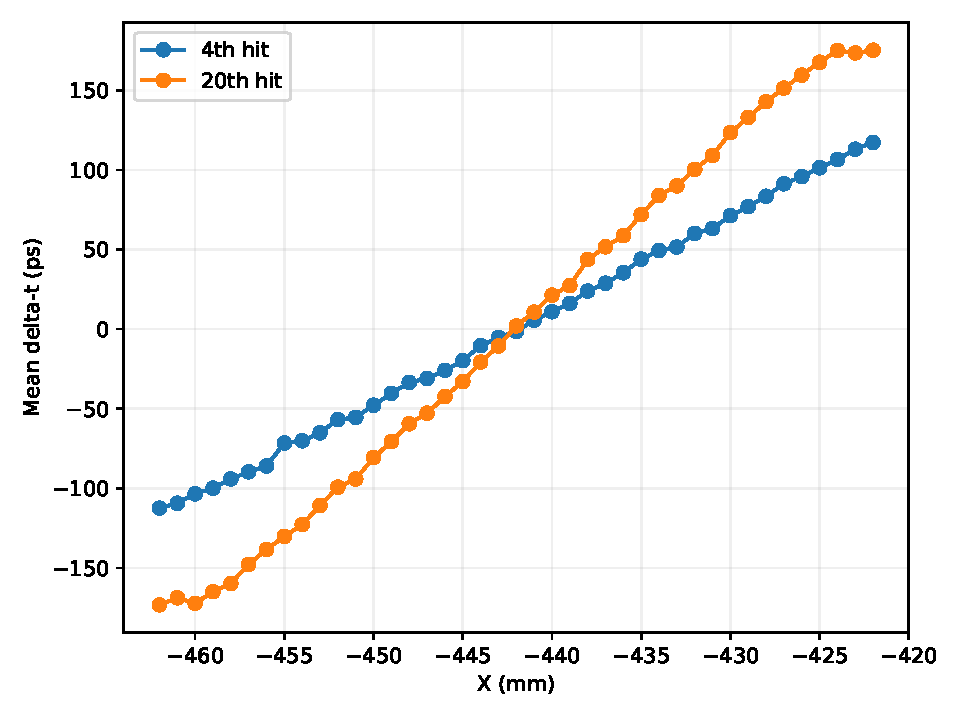
\includegraphics[width=.88\textwidth,height=.72\textheight,keepaspectratio]{../figures/mean_delta_4_20_vs_x.pdf}
\end{frame}
\begin{frame}{Non-Gaussian tails}
\centering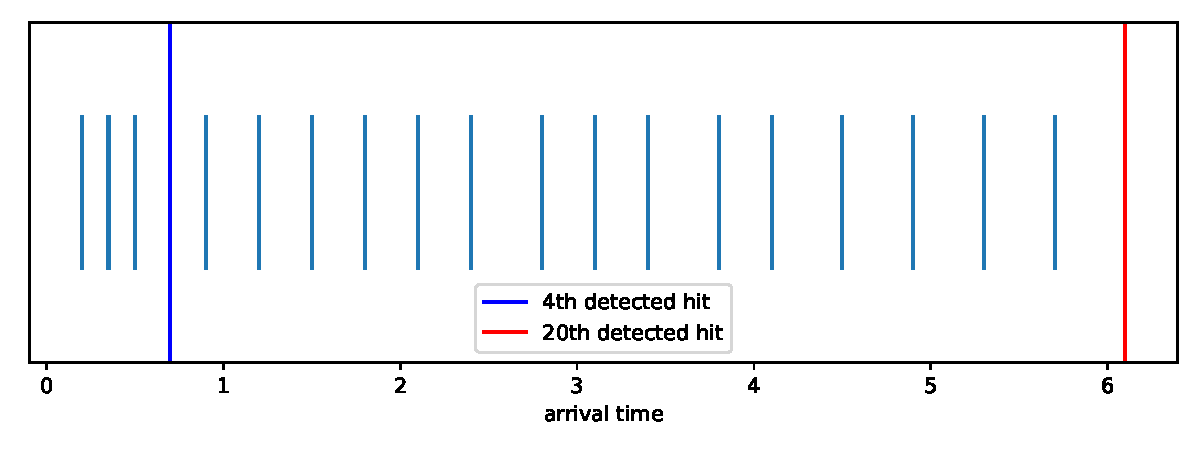
\includegraphics[width=.88\textwidth,height=.72\textheight,keepaspectratio]{../figures/order_statistic_schematic.pdf}
\end{frame}
\begin{frame}{REF1 comparison}
\centering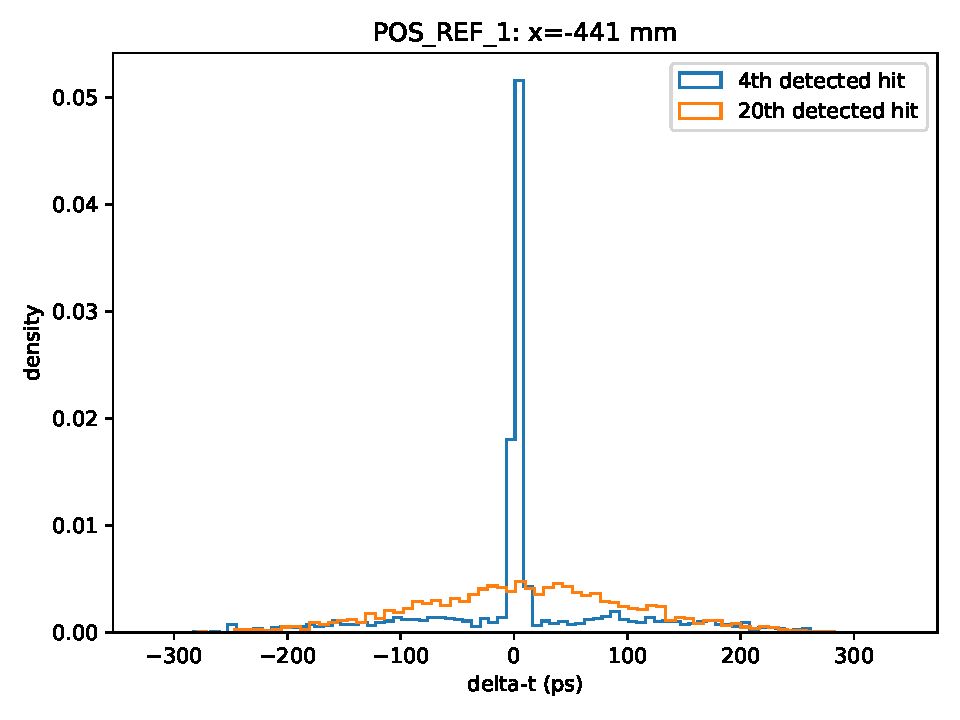
\includegraphics[width=.88\textwidth,height=.72\textheight,keepaspectratio]{../figures/pos_ref_1_delta_t_4_20.pdf}
\end{frame}
\begin{frame}{REF2 comparison}
\centering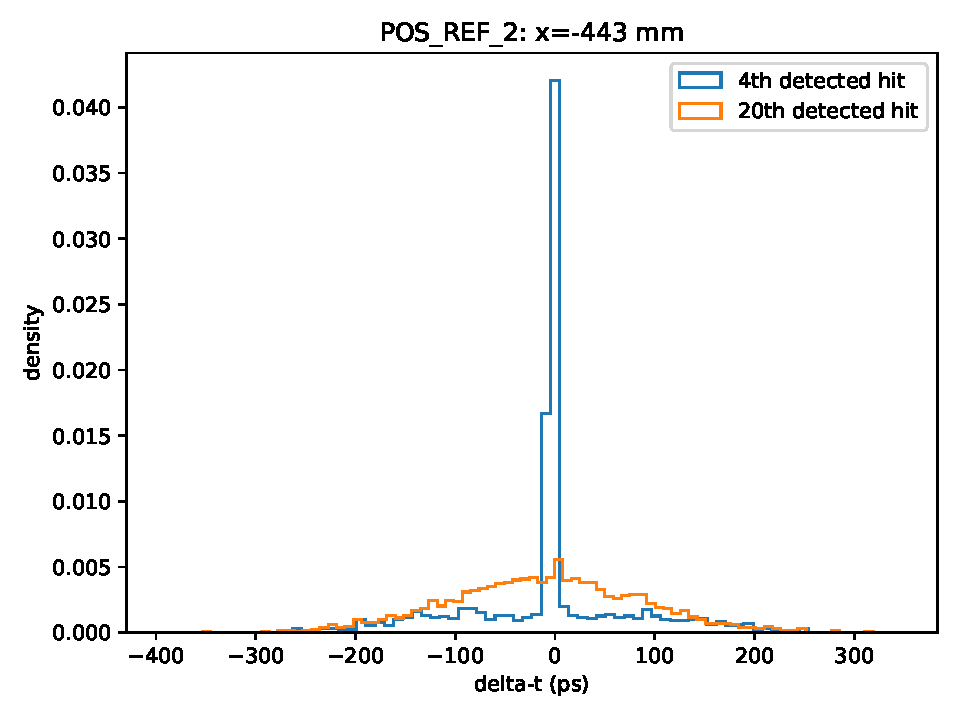
\includegraphics[width=.88\textwidth,height=.72\textheight,keepaspectratio]{../figures/pos_ref_2_delta_t_4_20.pdf}
\end{frame}
\begin{frame}{LOO position resolution}
\centering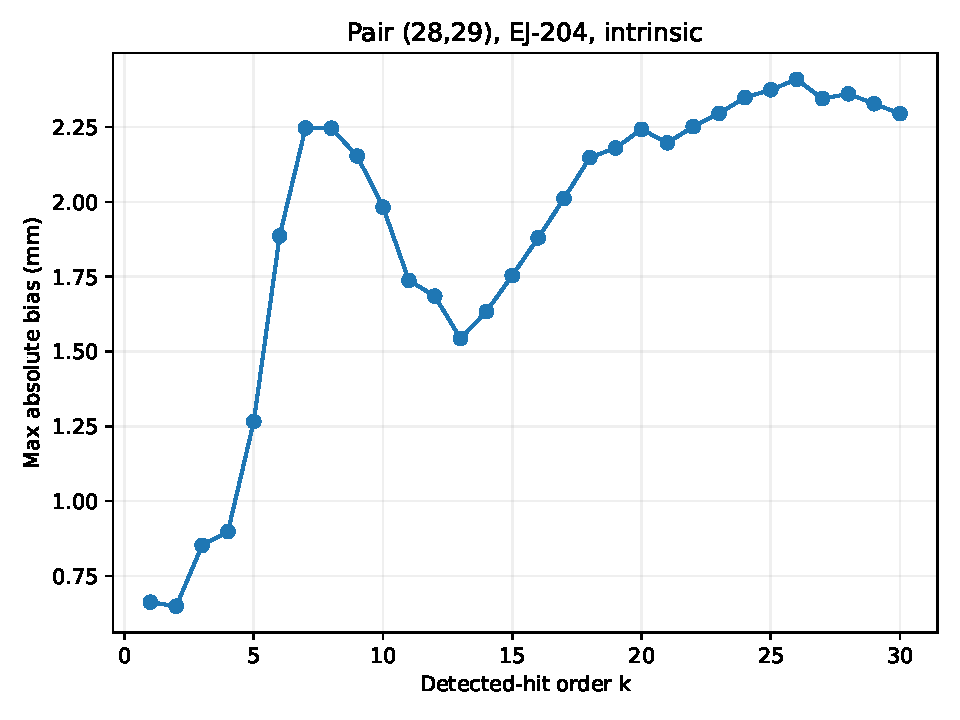
\includegraphics[width=.88\textwidth,height=.72\textheight,keepaspectratio]{../figures/threshold_bias.pdf}
\end{frame}
\begin{frame}{Bias and tails}
\centering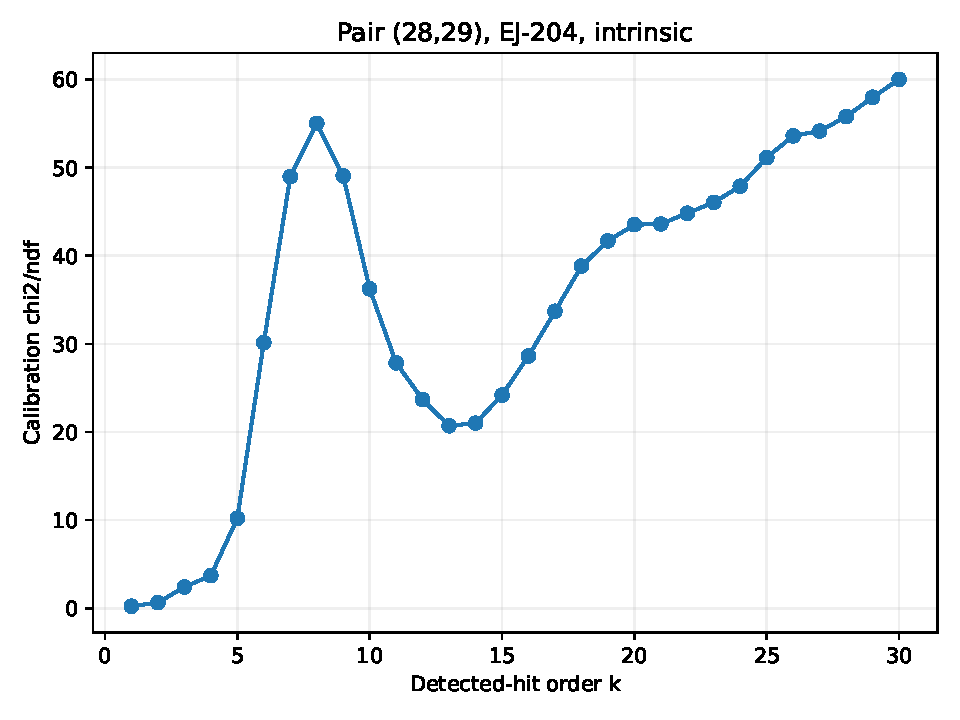
\includegraphics[width=.88\textwidth,height=.72\textheight,keepaspectratio]{../figures/threshold_chi2.pdf}
\end{frame}
\begin{frame}{Threshold efficiency}
\centering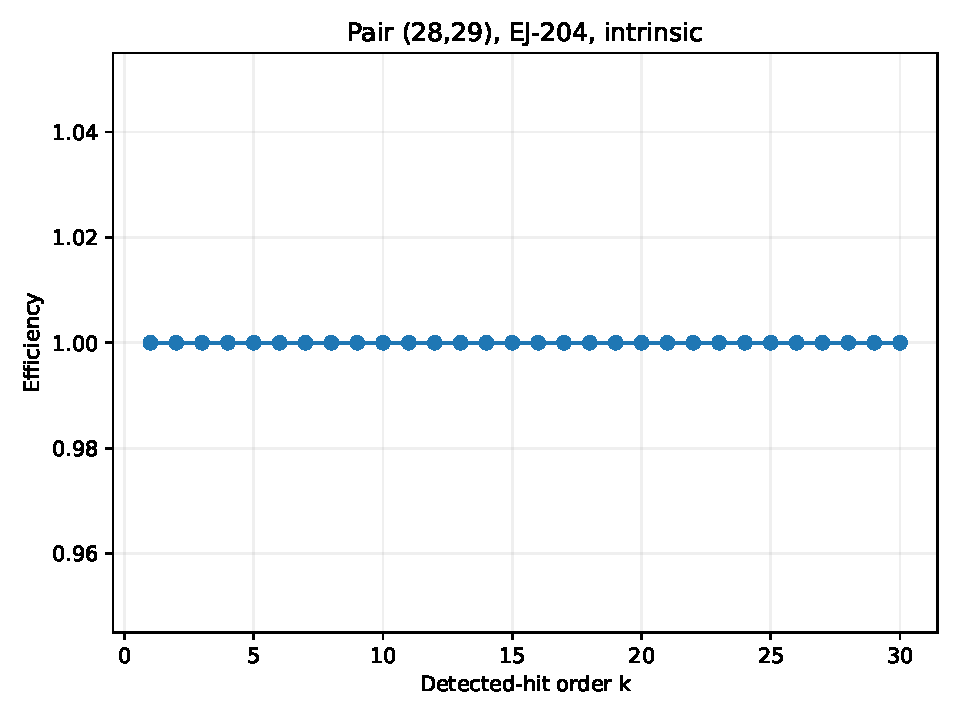
\includegraphics[width=.88\textwidth,height=.72\textheight,keepaspectratio]{../figures/threshold_efficiency.pdf}
\end{frame}
\begin{frame}{Threshold temporal width}
\centering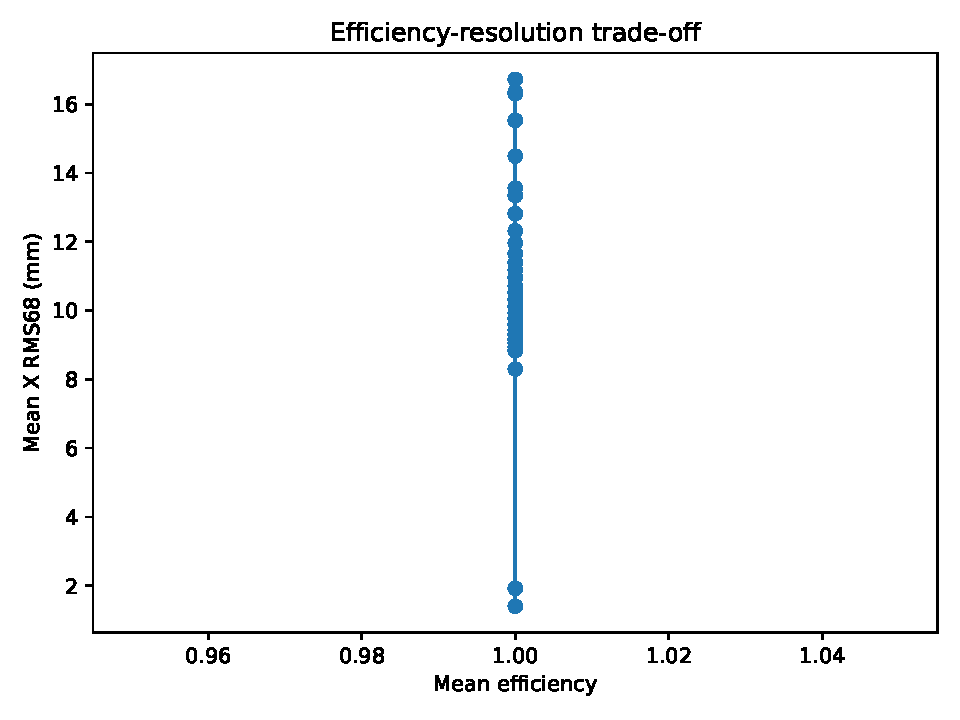
\includegraphics[width=.88\textwidth,height=.72\textheight,keepaspectratio]{../figures/threshold_pareto.pdf}
\end{frame}
\begin{frame}{Threshold position resolution}
\centering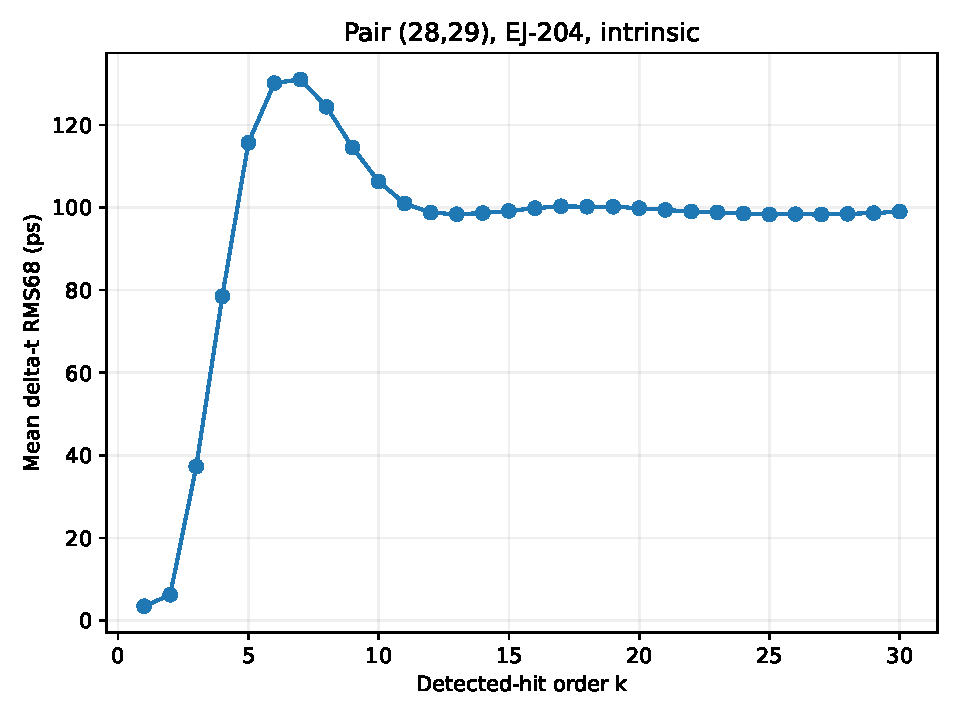
\includegraphics[width=.88\textwidth,height=.72\textheight,keepaspectratio]{../figures/threshold_sigma_dt.pdf}
\end{frame}
\begin{frame}{Pareto trade-off}
\centering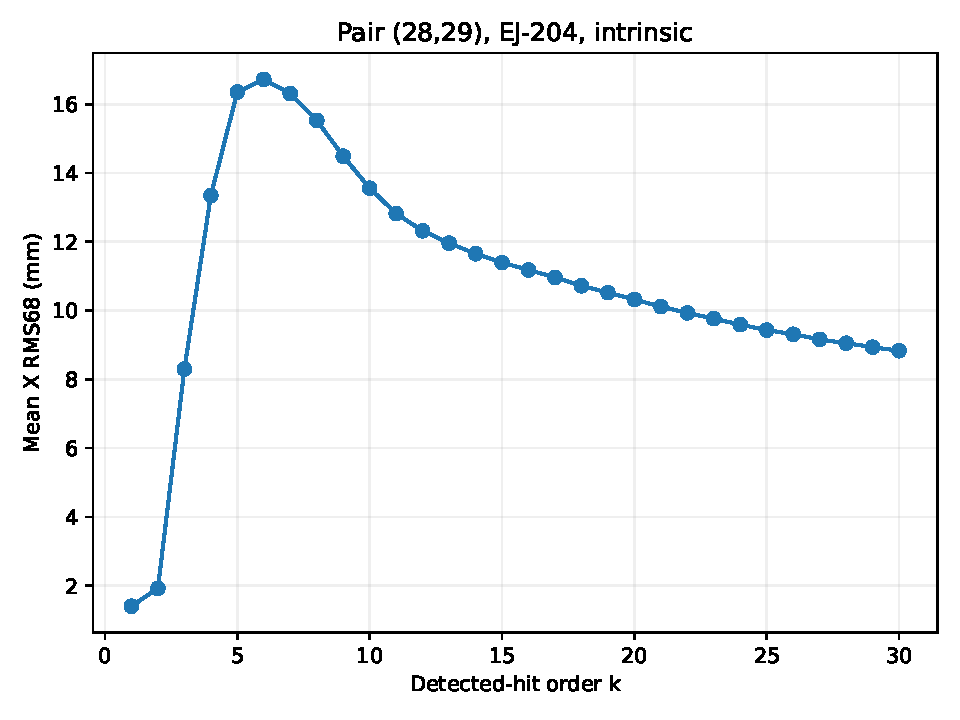
\includegraphics[width=.88\textwidth,height=.72\textheight,keepaspectratio]{../figures/threshold_sigma_x.pdf}
\end{frame}
\begin{frame}{Does 20th improve timing?}
\centering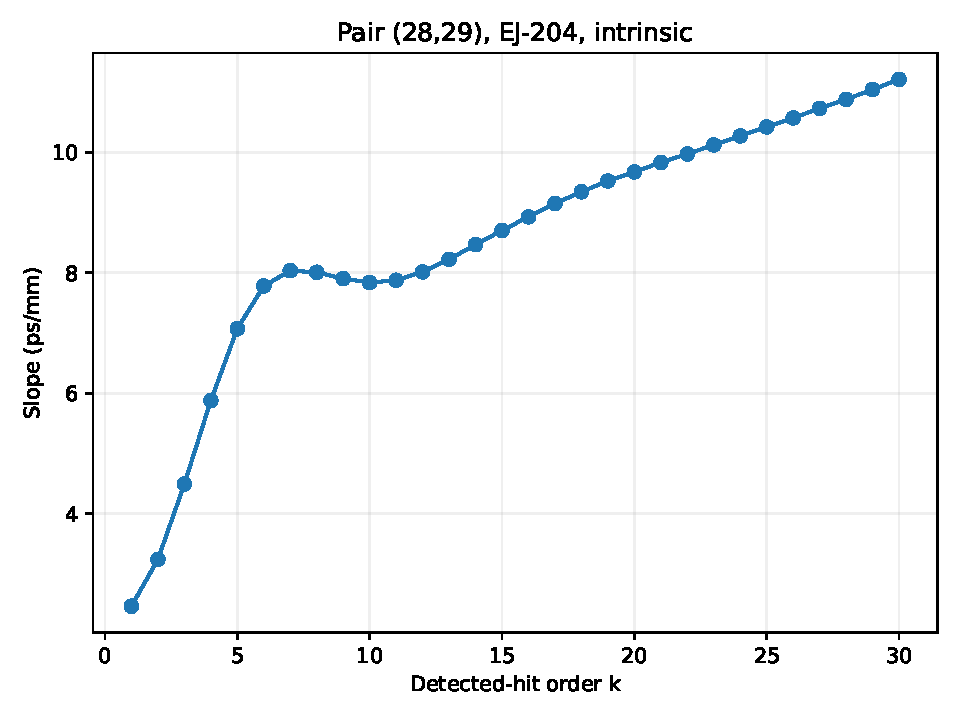
\includegraphics[width=.88\textwidth,height=.72\textheight,keepaspectratio]{../figures/threshold_slope.pdf}
\end{frame}
\begin{frame}{Common-time estimator}
\centering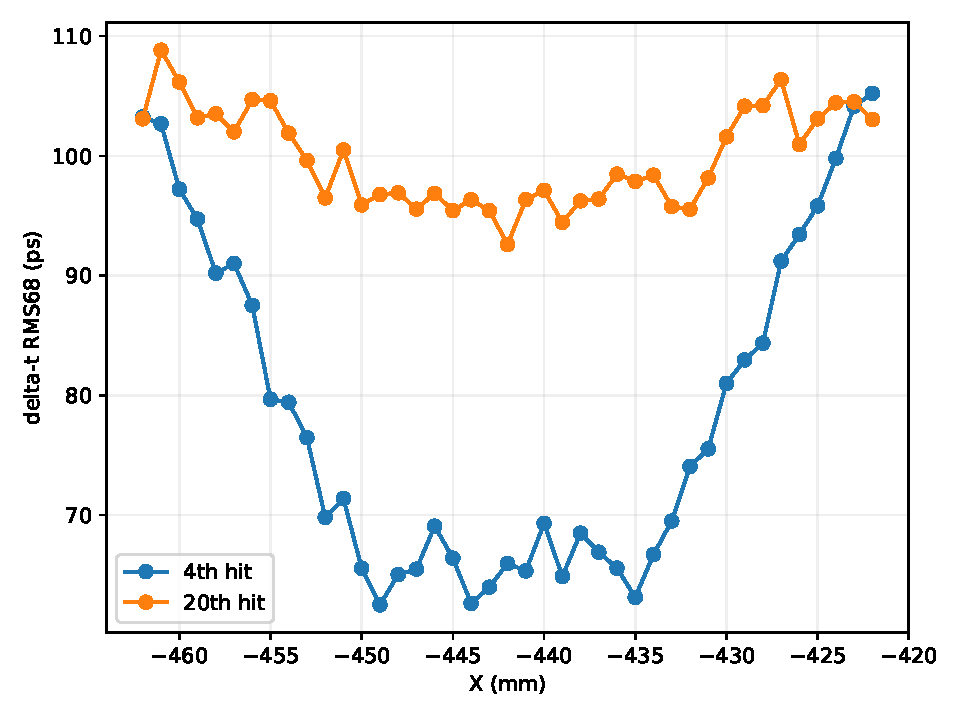
\includegraphics[width=.88\textwidth,height=.72\textheight,keepaspectratio]{../figures/timing_width_4_20_vs_x.pdf}
\end{frame}
\begin{frame}{Window dip geometry and light}
\centering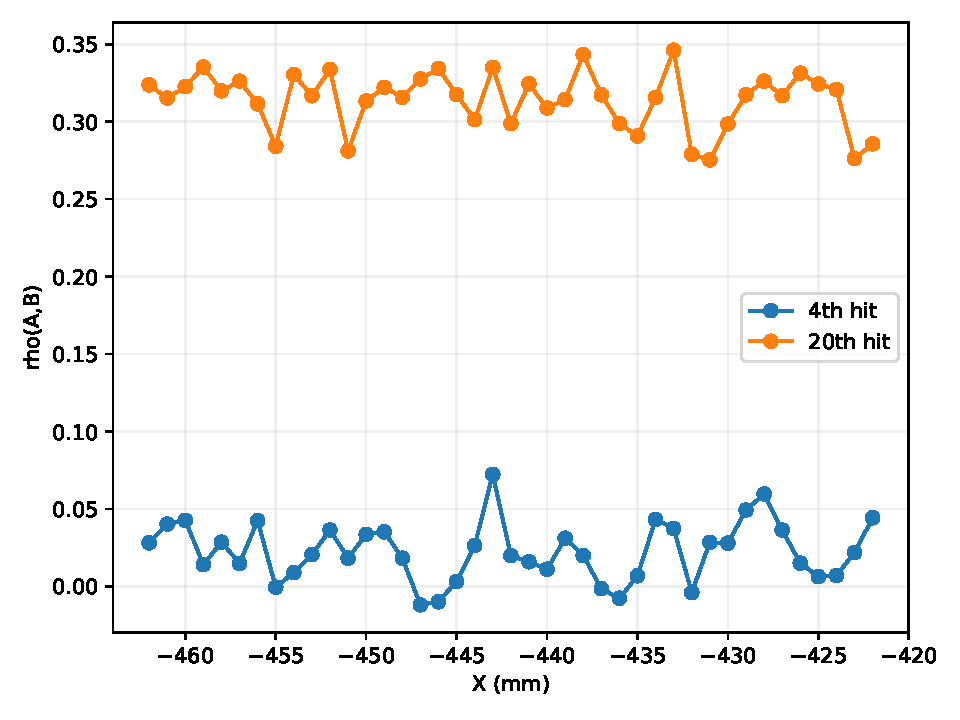
\includegraphics[width=.88\textwidth,height=.72\textheight,keepaspectratio]{../figures/correlation_ab_vs_x.pdf}
\end{frame}
\begin{frame}{Window dip timing}
\centering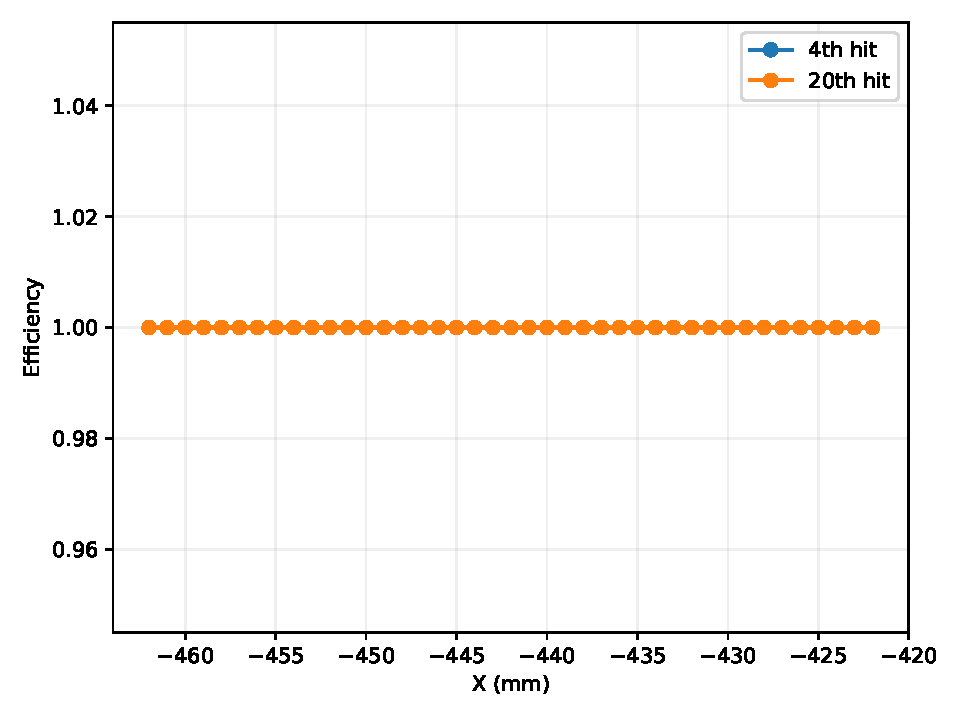
\includegraphics[width=.88\textwidth,height=.72\textheight,keepaspectratio]{../figures/efficiency_4_20_vs_x.pdf}
\end{frame}
\begin{frame}{Global EndTop context}
\centering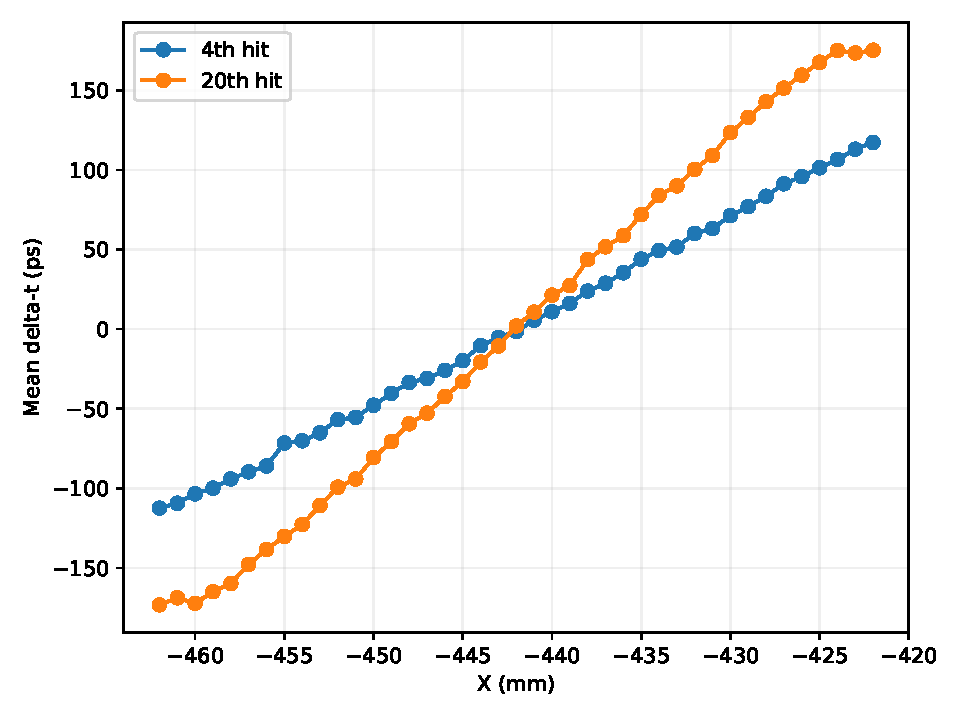
\includegraphics[width=.88\textwidth,height=.72\textheight,keepaspectratio]{../figures/mean_delta_4_20_vs_x.pdf}
\end{frame}
\begin{frame}{Gap and edge effects}
\centering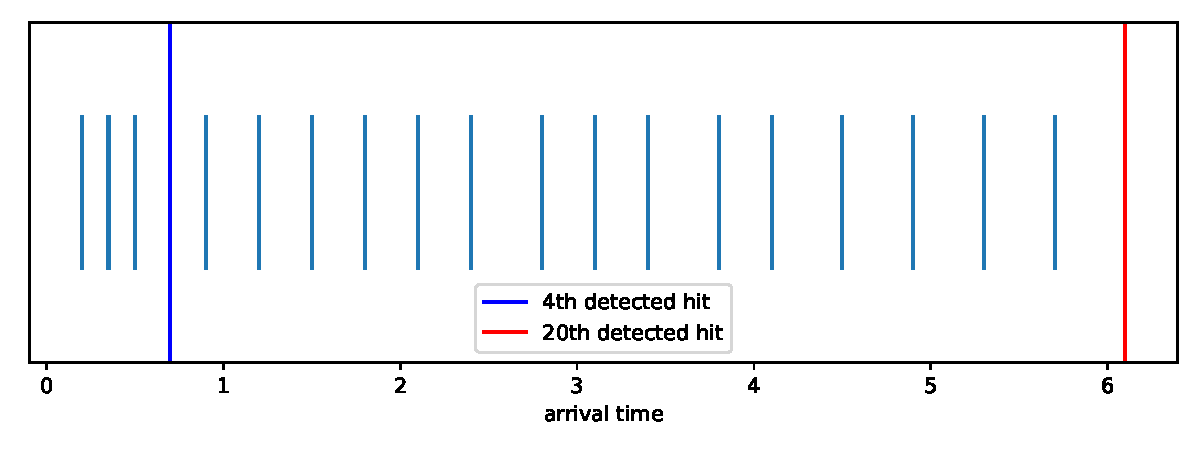
\includegraphics[width=.88\textwidth,height=.72\textheight,keepaspectratio]{../figures/order_statistic_schematic.pdf}
\end{frame}
\begin{frame}{Y=0 proxy}
\centering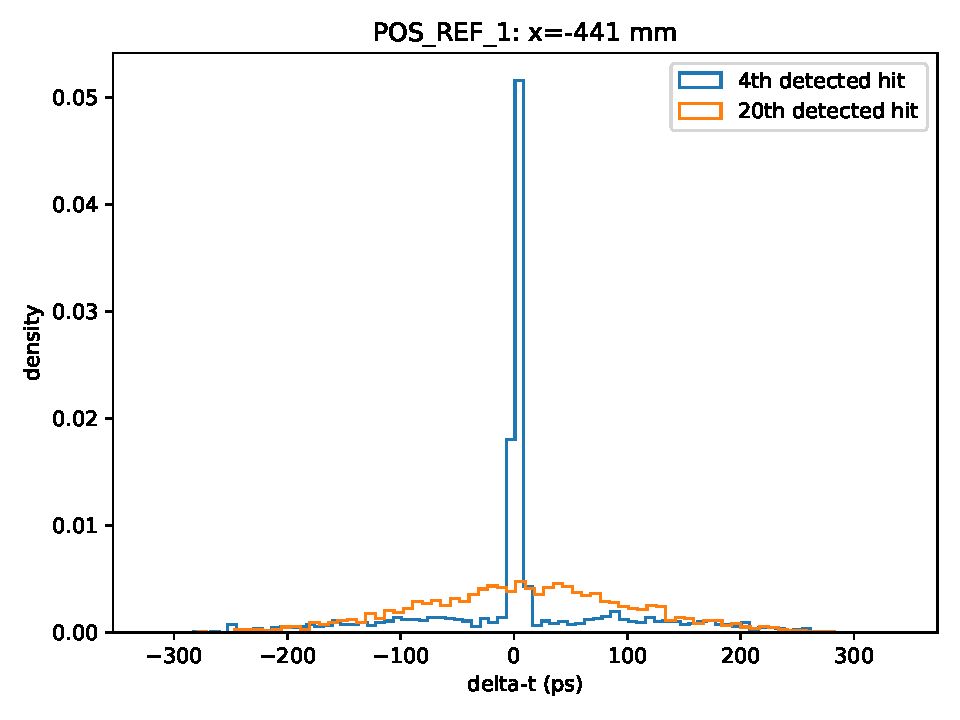
\includegraphics[width=.88\textwidth,height=.72\textheight,keepaspectratio]{../figures/pos_ref_1_delta_t_4_20.pdf}
\end{frame}
\begin{frame}{Comparison with Lv et al.}
\centering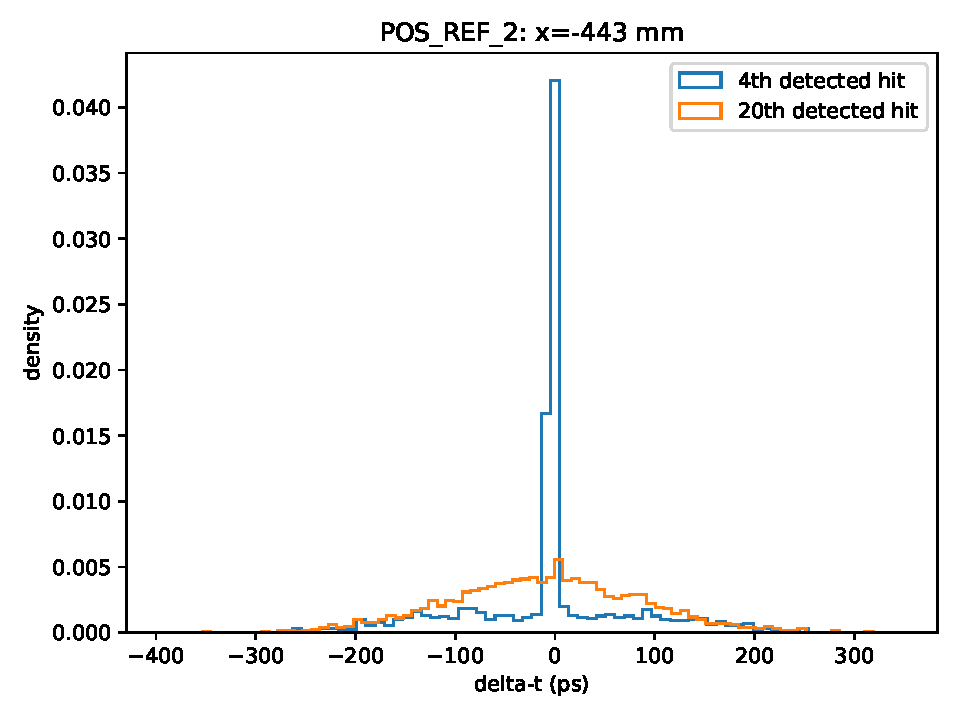
\includegraphics[width=.88\textwidth,height=.72\textheight,keepaspectratio]{../figures/pos_ref_2_delta_t_4_20.pdf}
\end{frame}
\begin{frame}{Timing budget}
\centering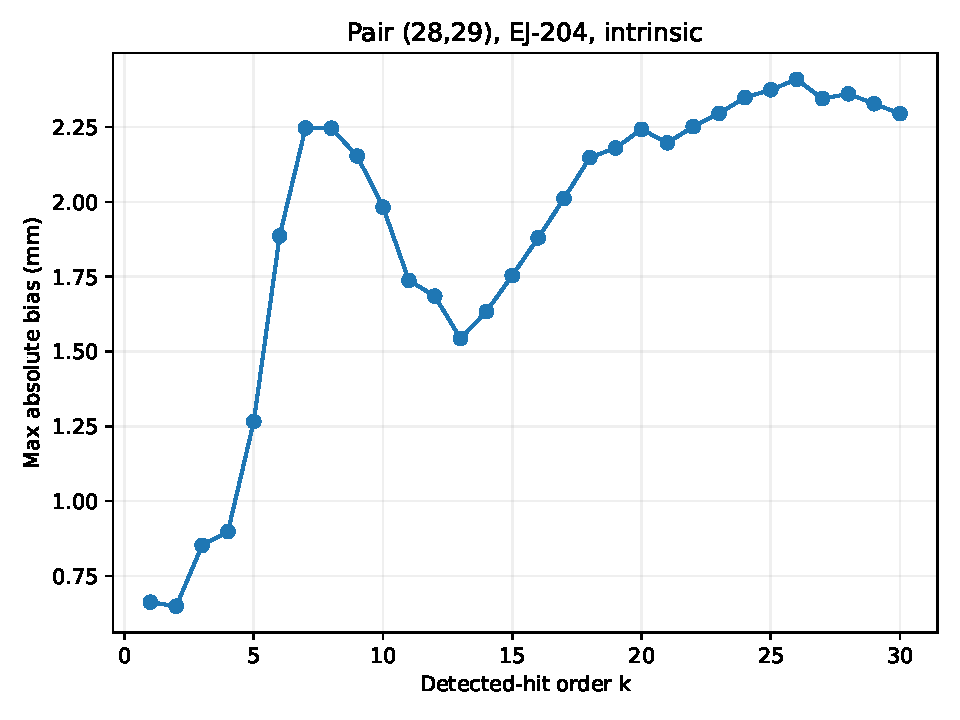
\includegraphics[width=.88\textwidth,height=.72\textheight,keepaspectratio]{../figures/threshold_bias.pdf}
\end{frame}
\begin{frame}{Conclusions}
\begin{itemize}
\item EXEC 11 4PE reproduction gate: \textbf{PASS}.
\item Native and matched samples coincide: 4PE and 20PE efficiencies are 100\%.
\item 20th-hit differential width: 99.8 ps, versus 78.5 ps for 4th hit.
\item Cross-validated X RMS68: 10.32 mm at 20PE, versus 13.34 mm at 4PE.
\item Higher thresholds improve X RMS68 here, while calibration nonlinearity rises.
\item Intrinsic simulation prediction; 20th detected hit is not waveform 20\% CFD.
\end{itemize}
\end{frame}
\appendix
\begin{frame}{Backup: Inventory}
\centering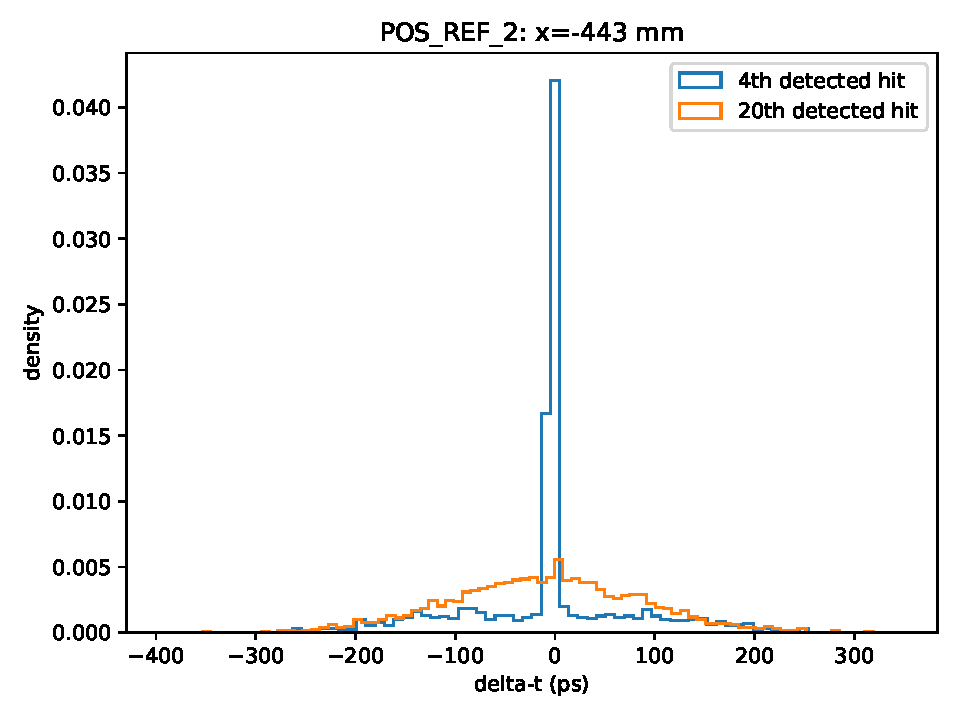
\includegraphics[width=.88\textwidth,height=.72\textheight,keepaspectratio]{../figures/pos_ref_2_delta_t_4_20.pdf}
\end{frame}
\begin{frame}{Backup: Schema}
\centering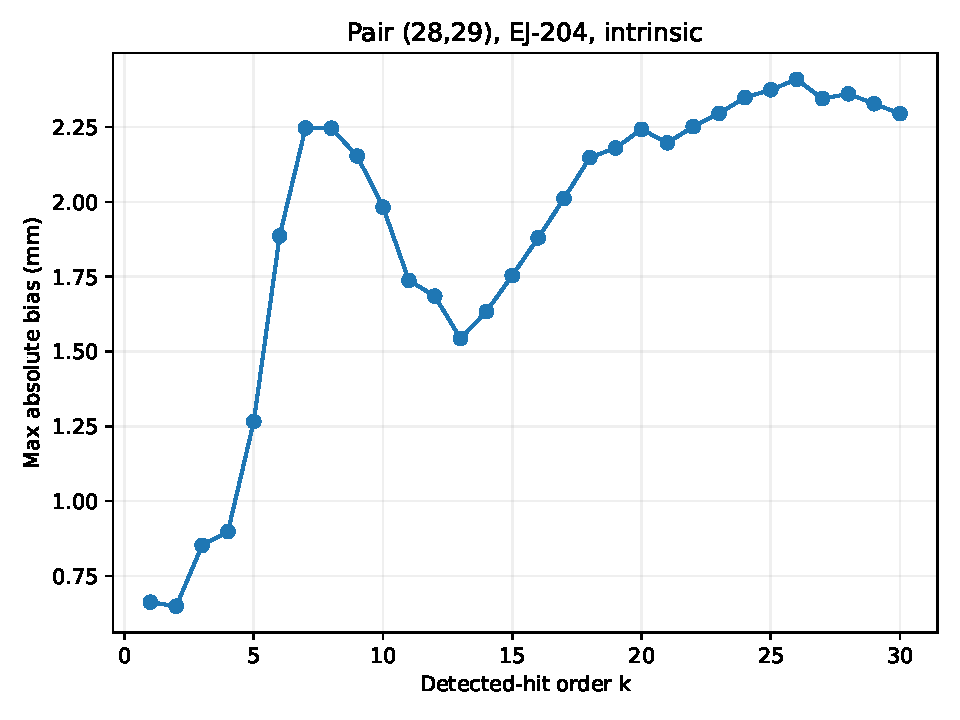
\includegraphics[width=.88\textwidth,height=.72\textheight,keepaspectratio]{../figures/threshold_bias.pdf}
\end{frame}
\begin{frame}{Backup: Builder tests}
\centering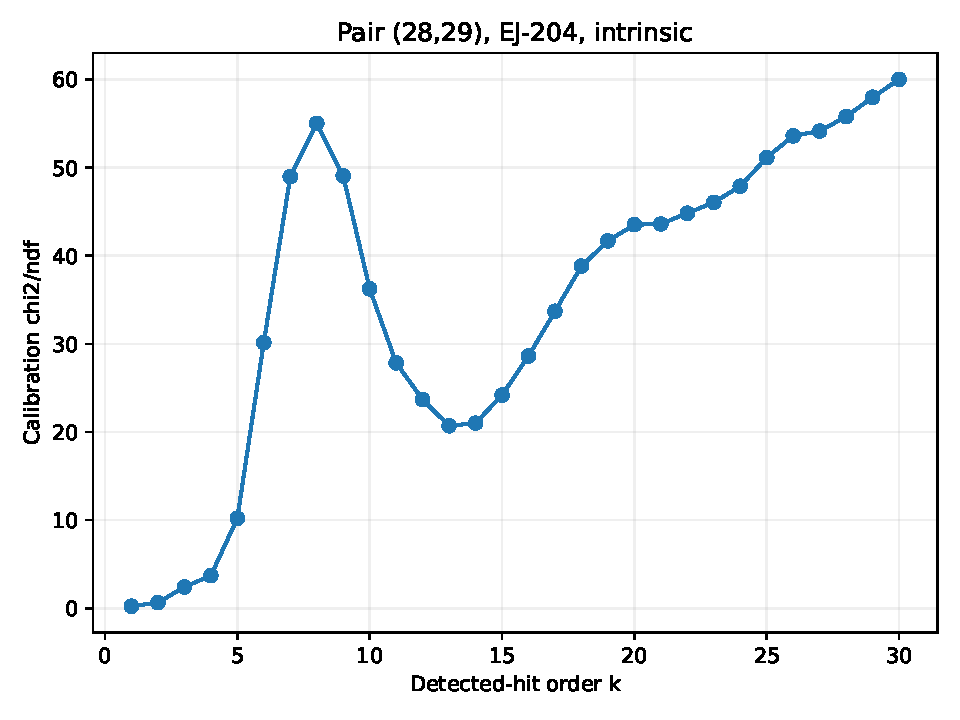
\includegraphics[width=.88\textwidth,height=.72\textheight,keepaspectratio]{../figures/threshold_chi2.pdf}
\end{frame}
\begin{frame}{Backup: Fit QA}
\centering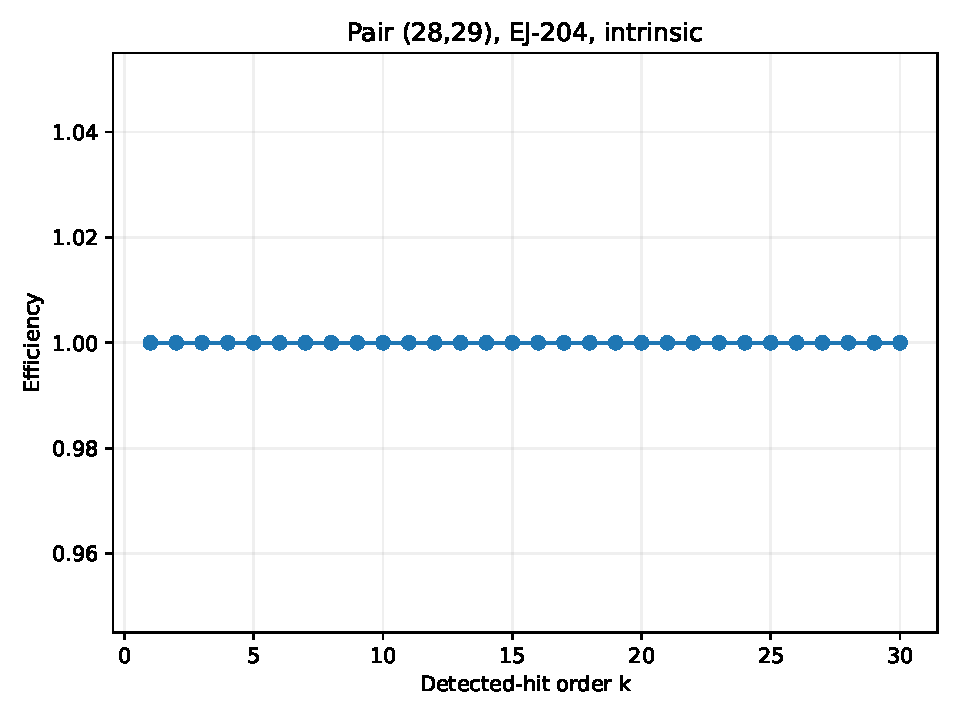
\includegraphics[width=.88\textwidth,height=.72\textheight,keepaspectratio]{../figures/threshold_efficiency.pdf}
\end{frame}
\begin{frame}{Backup: Threshold table}
\centering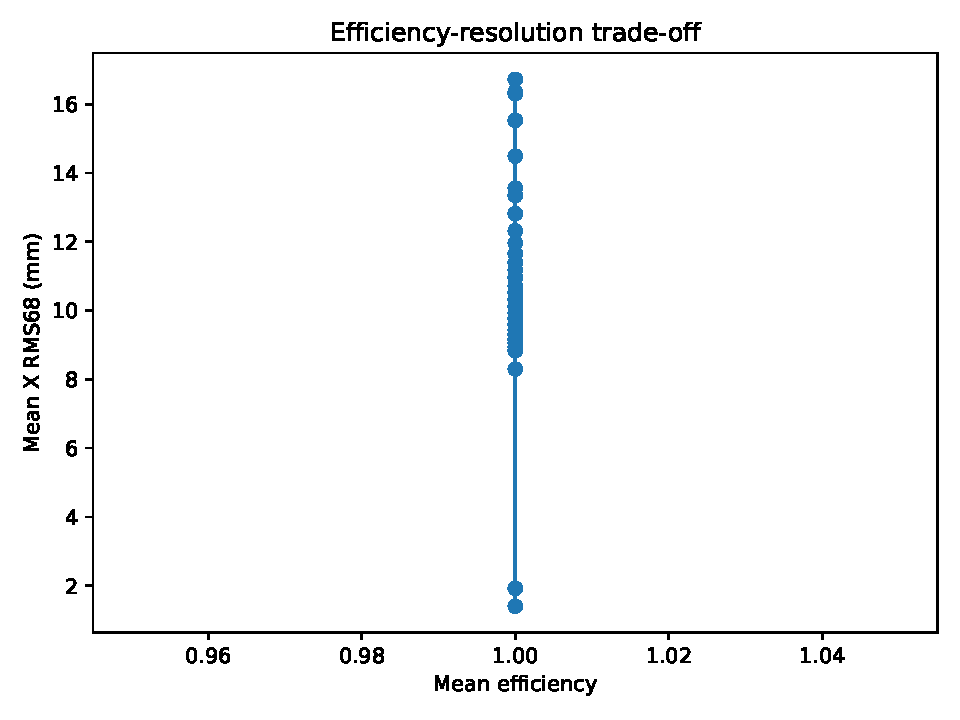
\includegraphics[width=.88\textwidth,height=.72\textheight,keepaspectratio]{../figures/threshold_pareto.pdf}
\end{frame}
\begin{frame}{Backup: Calibration covariance}
\centering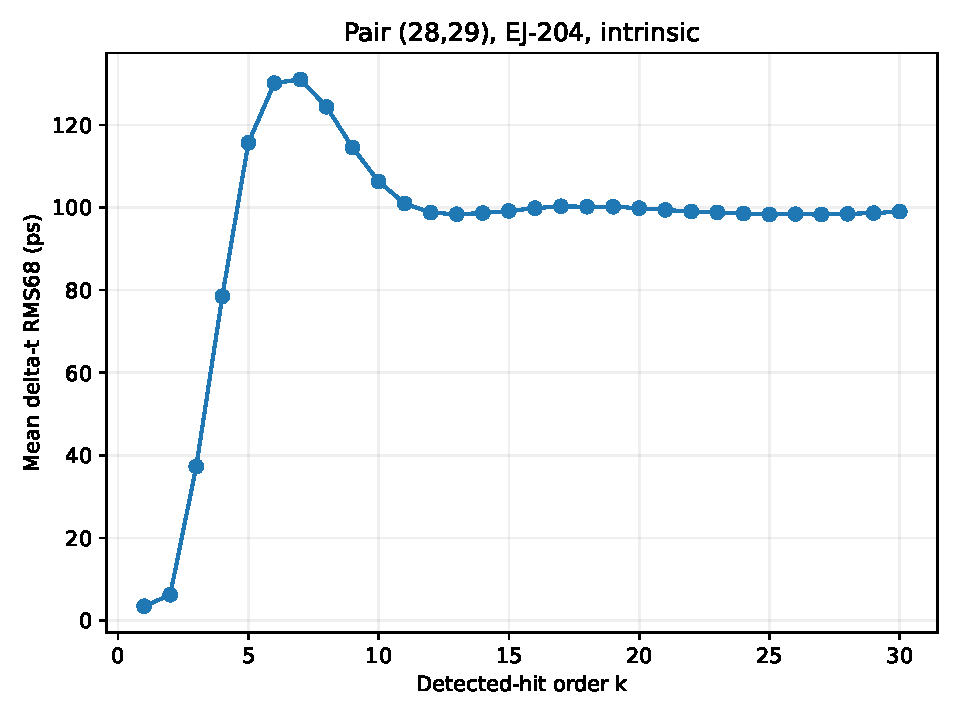
\includegraphics[width=.88\textwidth,height=.72\textheight,keepaspectratio]{../figures/threshold_sigma_dt.pdf}
\end{frame}
\begin{frame}{Backup: LOO details}
\centering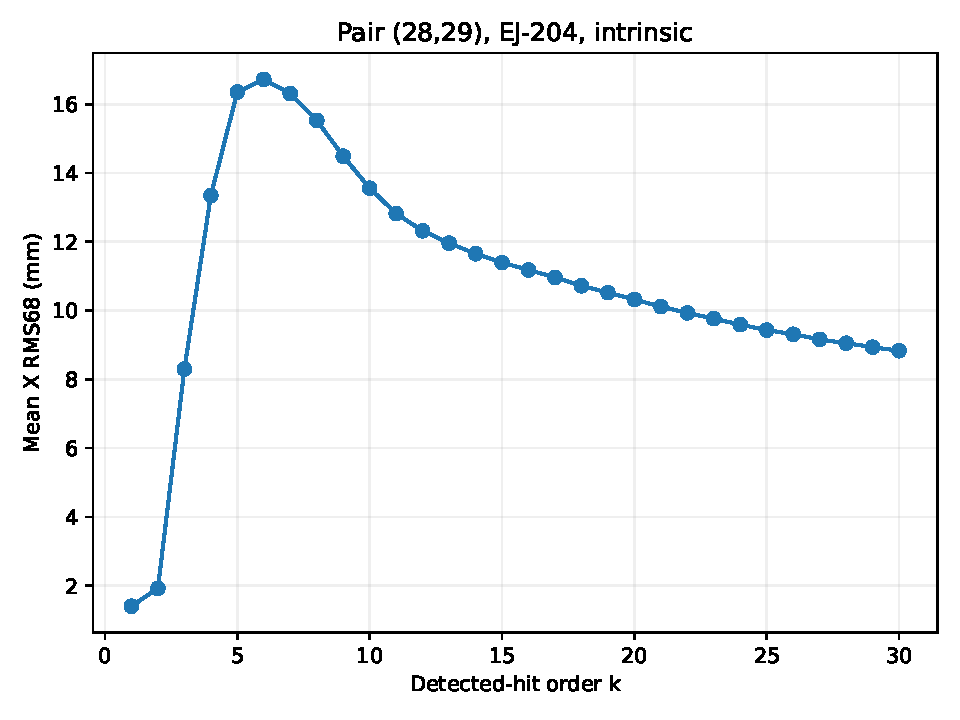
\includegraphics[width=.88\textwidth,height=.72\textheight,keepaspectratio]{../figures/threshold_sigma_x.pdf}
\end{frame}
\begin{frame}{Backup: Tail definitions}
\centering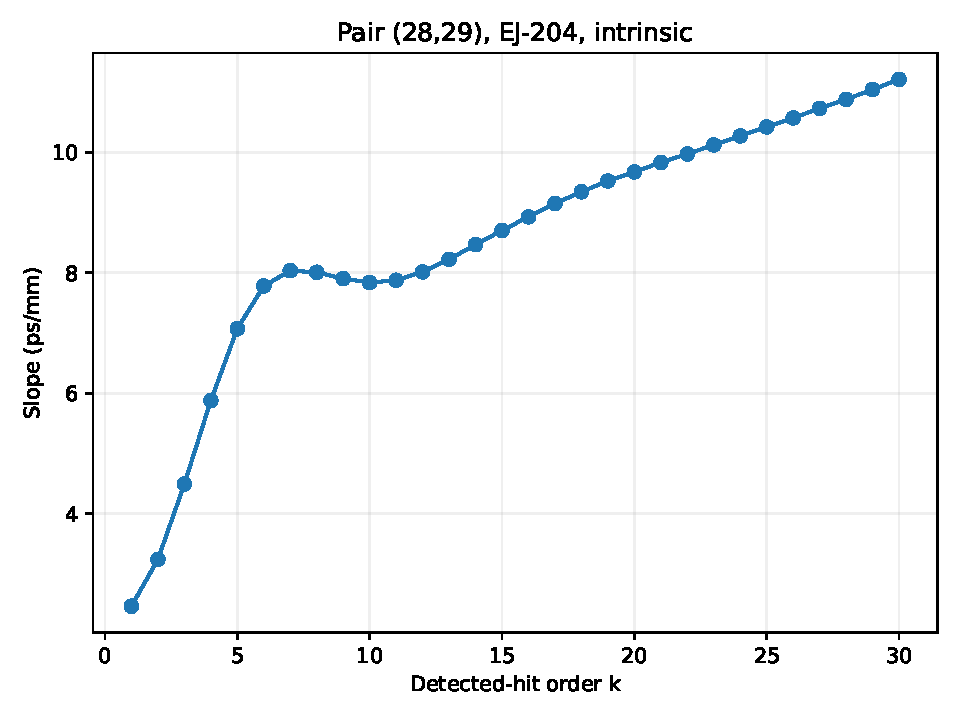
\includegraphics[width=.88\textwidth,height=.72\textheight,keepaspectratio]{../figures/threshold_slope.pdf}
\end{frame}
\begin{frame}{Backup: Window metadata}
\centering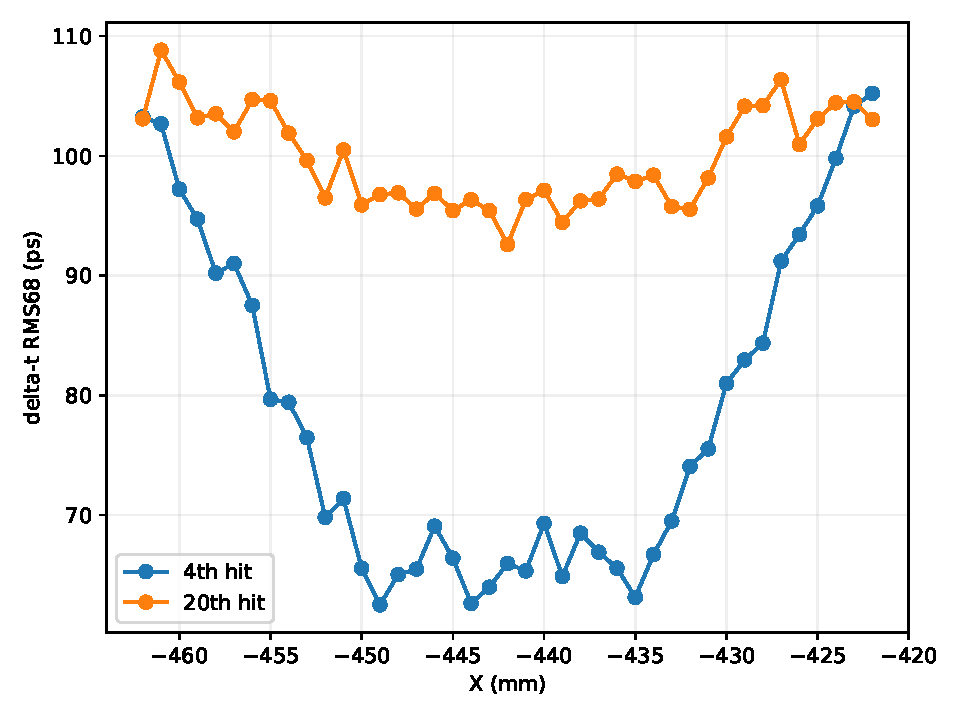
\includegraphics[width=.88\textwidth,height=.72\textheight,keepaspectratio]{../figures/timing_width_4_20_vs_x.pdf}
\end{frame}
\begin{frame}{Backup: Global methods}
\centering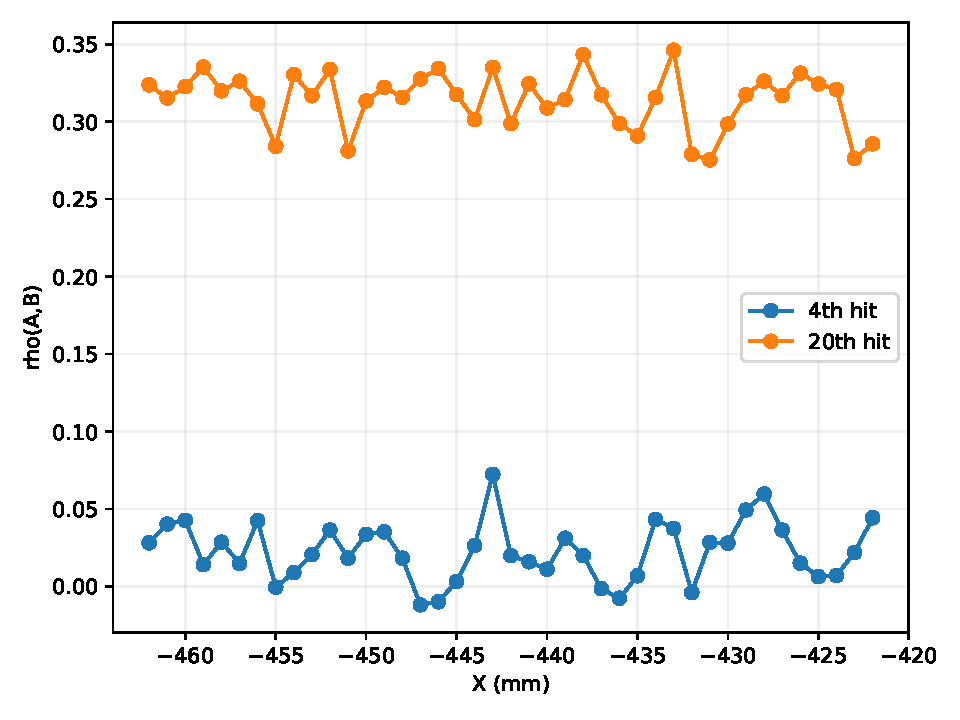
\includegraphics[width=.88\textwidth,height=.72\textheight,keepaspectratio]{../figures/correlation_ab_vs_x.pdf}
\end{frame}
\begin{frame}{Backup: Paper comparison}
\centering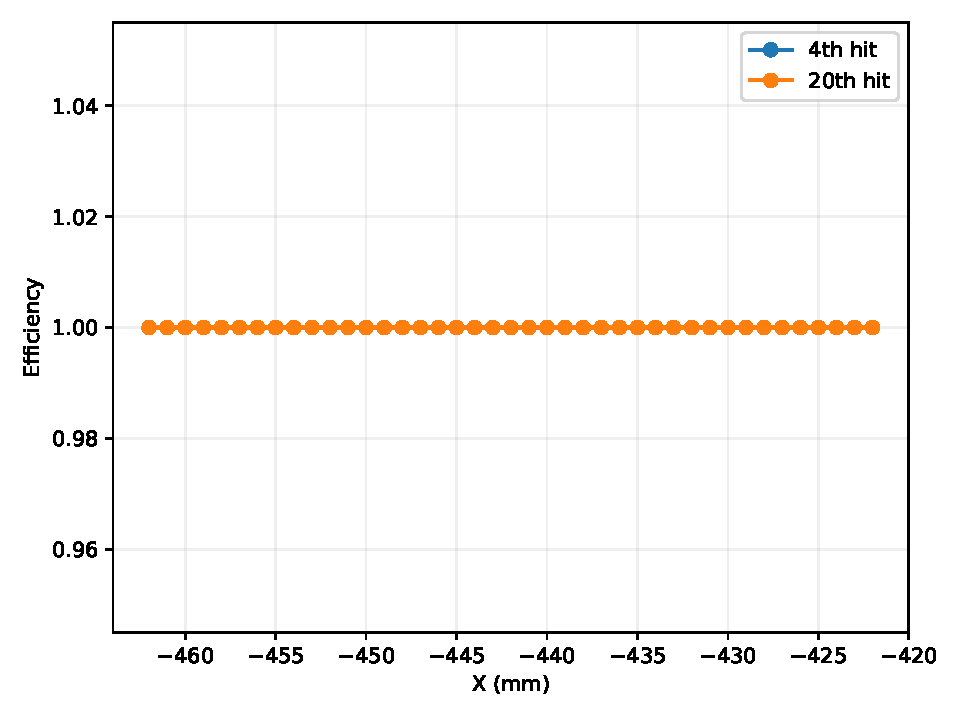
\includegraphics[width=.88\textwidth,height=.72\textheight,keepaspectratio]{../figures/efficiency_4_20_vs_x.pdf}
\end{frame}
\begin{frame}{Backup: Reproducibility}
\centering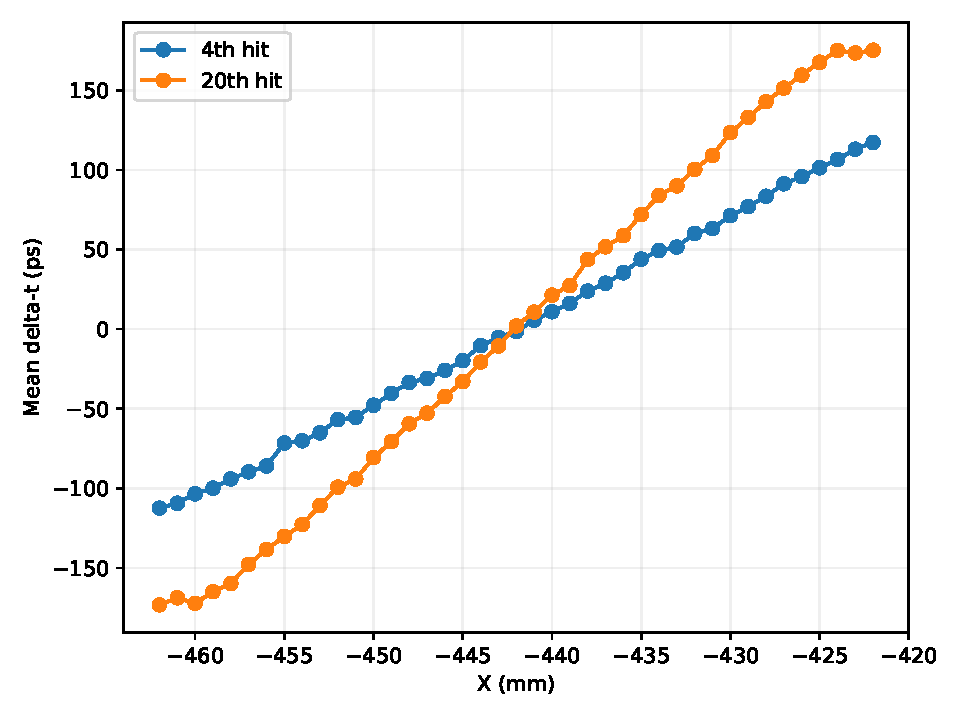
\includegraphics[width=.88\textwidth,height=.72\textheight,keepaspectratio]{../figures/mean_delta_4_20_vs_x.pdf}
\end{frame}
\end{document}
